\documentclass[a4paper, 11pt]{article}
\usepackage[margin=0.75in]{geometry}
\usepackage{graphicx, tabularx, hyperref, amsmath}
\usepackage[usenames,dvipsnames]{color,xcolor}
\usepackage{listings}
\usepackage{hyperref}
\usepackage[siunitx]{circuitikz}
\usepackage{booktabs}
\usepackage{pgfplotstable, pgfplots}
\renewcommand{\arraystretch}{1.2}
\usepackage{xepersian}
\settextfont[Scale=0.9]{Dibaj}
\setdigitfont[Scale=1]{Dibaj}

\lstset{
    basicstyle=\ttfamily\small,
    keywordstyle=\color{blue},
    commentstyle=\color{green!50!black},
    stringstyle=\color{red!70!black},
    numbers=left,
    numberstyle=\tiny,
    stepnumber=1,
    breaklines=true,
    frame=single
}


\begin{document}

\begin{center}
\textbf{{\huge گزارش‌کار آزمایش شمارهٔ
3:
اندازه‌گیری میدان مغناطیسی زمین، ضریب تراوایی مغناطیسی خلا و بررسی توزیع میدان
مغناطیسی پیچه‌های هلمهولتز
}}

\end{center}

\hrule
\noindent\begin{tabular}{rrl}
اعضای گروه: & ابوالفضل احمدی & 403172283\\
& نام و نام‌خانوادگی & 403001122
\end{tabular}\hfill
\begin{tabular}{rr}
تاریخ انجام آزمایش: & 24/08/1404 \\
دستیار آموزشی: &  \\
\end{tabular}\hfill
\begin{tabular}{rr}
گروه:  &  \\
زیرگروه: \lr{A} &  \\
\end{tabular}
\hrule


\section{اندازه‌گیری میدان مغناطیسی یک سیم‌پیچ دوتایی در جهت محوری در حالت $a=R$}

\begin{table}[h!]
\caption{مقادیر تجربی میدان مغناطیسی در حالت $a=R$}
\centering
\begin{tabular}{cc}
\hline
$D \;[\mathrm{cm}]$ & $B_H \;[\mathrm{mT}]$ \\
\hline
 $0$ & $1.49$ \\
$10$ & $1.42$ \\
$15$ & $1.26$ \\
$20$ & $1.00$ \\
$25$ & $0.73$ \\
$30$ & $0.50$ \\
$35$ & $0.35$ \\
$40$ & $0.24$ \\
$45$ & $0.18$ \\
$50$ & $0.13$ \\
\hline
\end{tabular}
\end{table}

\begin{figure}[h!]
\centering
\pgfplotsset{
    width=9cm,
    height=5cm,
    scale only axis,
    tick align = outside,
    yticklabel style={/pgf/number format/fixed},  
}
\begin{tikzpicture}
\begin{axis}[
    title=\rl{{میدان $B_H$ برحسب جابجایی $D$}},
    xlabel={
        \lr{[$\mathrm{cm}$]} جابجایی $D$
    },
    ylabel={
        \lr{[$\mathrm{mT}$]} میدان $B_H$
    },
    ymin=0, ymax=1.6,
    xmin=0, xmax=55,
    ytick distance=0.2,
    xtick distance=5,
    legend pos=north east,
    ymajorgrids=true,
    xmajorgrids=true,
    grid style=dashed,
    grid=both,
    minor y tick num=1,
    minor x tick num=1,
    xticklabel style={
                /pgf/number format/fixed,
                /pgf/number format/precision=0,
                /pgf/number format/fixed zerofill
            },
]

\addplot[
mark=square, smooth
]
coordinates {
(0, 1.49)
(10, 1.42)
(15, 1.26)
(20, 1.00)
(25, 0.73)
(30, 0.50)
(35, 0.35)
(40, 0.24)
(45, 0.18)
(50, 0.13)
};

\end{axis}
\end{tikzpicture}
\end{figure}



\subsection{بحث دربارهٔ تفاوت نمودار تجربی و نمودار تئوری میدان برای \texorpdfstring{$a = \tfrac{R}{2}$}{a=R/2}}

در آرایش استاندارد سیم‌پیچ‌های هلمهولتز، فاصلهٔ بین دو سیم‌پیچ برابر شعاع آن‌ها است:
\[
a = R
\]
این آرایش باعث می‌شود که مشتق دوم میدان مغناطیسی در مرکز صفر شود:
\[
\frac{d^2 B}{dx^2}\bigg|_{x=0} = 0
\]
و در نتیجه میدان در ناحیهٔ مرکزی تقریباً یکنواخت و «تخت» باشد. به همین دلیل نمودار میدان برحسب جابجایی در حالت هلمهولتز، در اطراف مرکز یک ناحیهٔ یکنواخت دارد.

اما در آزمایش حاضر فاصلهٔ بین دو سیم‌پیچ به صورت
\[
a = \frac{R}{2}
\]
انتخاب شده است. این آرایش دیگر ویژگی‌های هلمهولتز را ندارد و میدان مغناطیسی حاصل کاملاً متفاوت رفتار می‌کند. در چنین حالتی میدان مغناطیسی روی محور به صورت مجموع میدان دو حلقه است:
\[
B(D) \propto 
\frac{1}{\left(R^{2} + (D - \tfrac{R}{4})^{2}\right)^{3/2}}
+
\frac{1}{\left(R^{2} + (D + \tfrac{R}{4})^{2}\right)^{3/2}}.
\]

در این ساختار، میدان در مرکز (\(D=0\)) دارای بیشینه است، اما برخلاف آرایش هلمهولتز، مقدار میدان به‌سرعت و به‌شکل غیرخطی با افزایش فاصله کاهش می‌یابد. به همین دلیل نمودار حاصل یک قلهٔ تیز در مرکز دارد و فاقد ناحیهٔ تخت است. این رفتار نشان می‌دهد که گرادیان میدان بسیار زیاد است و تغییرات میدان شدیدتر از حالت هلمهولتز می‌باشد. [ضمیمه آ]
\begin{figure}[h!]
\centering
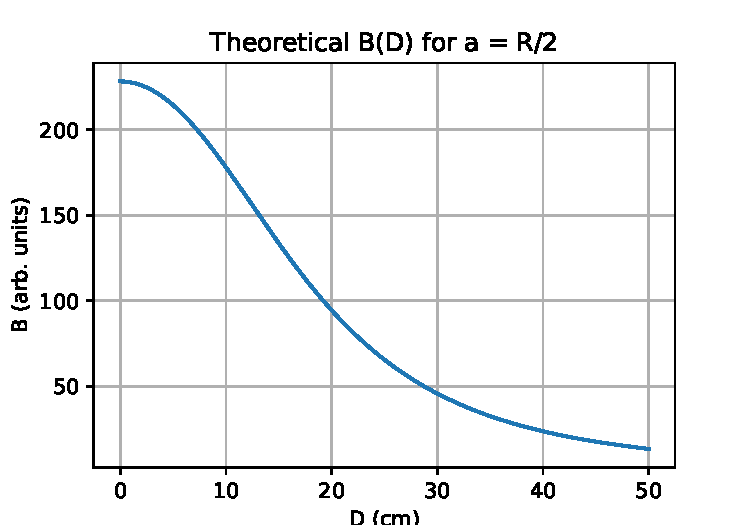
\includegraphics{fig-01.pdf}
\end{figure}


به‌طور خلاصه، تفاوت اصلی بین نمودار تجربی و نمودار میدان هلمهولتز استاندارد به‌صورت زیر بیان می‌شود:
\begin{itemize}
    \item در حالت هلمهولتز \((a=R)\)، میدان در مرکز یکنواخت است و نمودار ناحیهٔ تخت دارد.
    \item در حالت آزمایش \((a=\tfrac{R}{2})\)، یکنواختی میدان از بین می‌رود و میدان شکل قله‌ای و شدیداً غیریکنواخت پیدا می‌کند.
    \item مقدار میدان در مرکز بزرگ‌تر بوده و افت آن با فاصله بسیار سریع‌تر از حالت هلمهولتز اتفاق می‌افتد.
\end{itemize}

بنابراین کم‌بودن فاصلهٔ بین دو سیم‌پیچ باعث می‌شود میدان مغناطیسی روی محور رفتار تئوری متفاوتی داشته باشد و نمودار تجربی نیز همین رفتار را نشان می‌دهد.

\subsection{رفتار میدان سیم‌پیچ‌ها در جهت شعاعی \texorpdfstring{$r$}{r}}

برای یک سیم‌پیچ دایره‌ای، میدان مغناطیسی در مرکز بیشترین مقدار را دارد و با حرکت در جهت شعاعی \(r\)، یعنی در همان صفحهٔ سیم‌پیچ و دور شدن از محور تقارن، میدان مغناطیسی کاهش می‌یابد. این کاهش به دلیل تغییر زاویهٔ عناصر جریان نسبت به نقطهٔ مشاهده و همچنین افزایش فاصلهٔ آن نقطه از سیم‌پیچ است.

از نظر تئوری، میدان در جهت شعاعی متناسب با تابعی کاهشی از مرتبهٔ بالا است. رابطهٔ دقیق میدان در صفحهٔ سیم‌پیچ (در نقطه‌ای با فاصلهٔ شعاعی \(r\)) برای یک سیم‌پیچ با شعاع \(R\) چنین نوشته می‌شود:
\begin{equation}
B(r)
=
\frac{\mu_0 n I}{2\pi}
\frac{1}{\sqrt{(R+r)^2 \, (R-r)}}
\, K\!\left( \frac{4 R r}{(R+r)^2} \right),
\end{equation}
که در آن \(K\) انتگرال کامل بیضوی نوع اول است. این رابطه نشان می‌دهد که رفتار میدان در صفحهٔ سیم‌پیچ وابستگی تحلیلی پیچیده‌ای دارد.

با این حال، ویژگی کلی میدان در جهت \(r\) روشن است:
\begin{itemize}
    \item میدان در مرکز (\(r=0\)) بیشینه است.
    \item با دور شدن از مرکز، میدان به‌سرعت کاهش می‌یابد.
    \item برای \(r \approx R\)، میدان تقریباً به صفر میل می‌کند.
    \item افت میدان نسبت به حالت محوری بسیار سریع‌تر است.
\end{itemize}

بنابراین از نظر فیزیکی انتظار داریم میدان سیم‌پیچ‌ها در جهت شعاعی \(r\) یک رفتار به‌شدت کاهشی داشته باشد و تنها در نزدیکی مرکز (نزدیک محور) مقدار قابل‌توجهی باقی بماند.

\subsection{انتظار از اندازه‌گیری میدان برای مقادیر منفی \texorpdfstring{$D$}{D}}

چیدمان دو سیم‌پیچ به‌صورت کاملاً متقارن نسبت به مرکز دستگاه است؛ یک سیم‌پیچ در موقعیت
\(\,+\tfrac{a}{2}\,\)
و دیگری در
\(\,-\tfrac{a}{2}\,\)
بر روی محور قرار دارد. بنابراین میدان مغناطیسی حاصل روی محور باید نسبت به نقطهٔ
\(\,D=0\,\)
دارای تقارن زوج باشد.

رابطهٔ میدان روی محور برای دو سیم‌پیچ هم‌محور چنین است:
\begin{equation}
B(D)
=
\frac{\mu_0 n I R^2}{2}
\left[
\frac{1}{\left(R^2 + (D - \tfrac{a}{2})^2\right)^{3/2}}
+
\frac{1}{\left(R^2 + (D + \tfrac{a}{2})^2\right)^{3/2}}
\right].
\end{equation}

اگر به‌جای \(\,D\) مقدار \(-D\) را قرار دهیم، خواهیم داشت:
\begin{align}
B(-D)
&=
\frac{\mu_0 n I R^2}{2}
\left[
\frac{1}{\left(R^2 + (-D - \tfrac{a}{2})^2\right)^{3/2}}
+
\frac{1}{\left(R^2 + (-D + \tfrac{a}{2})^2\right)^{3/2}}
\right].
\end{align}

چون:
\[
(-D \pm \tfrac{a}{2})^2 = (D \mp \tfrac{a}{2})^2,
\]
نتیجه می‌گیریم:
\begin{equation}
B(-D) = B(D).
\end{equation}

بنابراین از دیدگاه تئوری میدان تابعی زوج از \(D\) است و نتیجهٔ مهم زیر حاصل می‌شود:
\begin{itemize}
    \item میدان در \(-D\) دقیقاً برابر میدان در \(+D\) است.
    \item نمودار میدان نسبت به محور عمودی \(D=0\) کاملاً متقارن خواهد بود.
    \item اگر مقادیر میدان برای \(D>0\) اندازه‌گیری شده باشند، مقادیر مورد انتظار برای \(D<0\) باید تصویر آینه‌ای همان نقاط باشند.
\end{itemize}

هرگونه عدم تقارن قابل توجه میان \(B(D)\) و \(B(-D)\) در اندازه‌گیری واقعی معمولاً ناشی از عواملی مانند ناهم‌محوری سیم‌پیچ‌ها، ناهمگنی محیط، خطای قرائت یا جای‌گذاری نادرست حسگر میدان است.

\section{محاسبه ضریب نفوذپذیری مغناطیسی}


\begin{table}[h!]
\caption{مقادیر تجربی برای محاسبه ضریب نفوذپذیری مغناطیسی}
\centering
\begin{tabular}{cc}
\hline
$I \;[\mathrm{A}]$ & $B_H \;[\mathrm{mT}]$ \\
\hline
 $0.2$ & $0.13$ \\
 $0.4$ & $0.28$ \\
 $0.6$ & $0.45$ \\
 $0.8$ & $0.61$ \\
 $1.0$ & $0.79$ \\
$1.23$ & $1.01$ \\
$1.43$ & $1.18$ \\
$1.65$ & $1.35$ \\
$1.77$ & $1.44$ \\
\hline
\end{tabular}
\end{table}

\subsection{محاسبات برازش خطی}
برای داده‌های جدول $B_H$ برحسب $I$، از روش حداقل مربعات برای یافتن معادله خط استفاده شد. معادله خط به صورت زیر است:
$$
y = mx + c
$$
که در آن:
 $m$ شیب خط است و
 $c$ عرض از مبدأ است.

داده‌های جدول:
$$
x = I = [0.2, 0.4, 0.6, 0.8, 1.0, 1.23, 1.43, 1.65, 1.77]
$$
$$
y = B_H = [0.13, 0.28, 0.45, 0.61, 0.79, 1.01, 1.18, 1.35, 1.44]
$$

محاسبه مقادیر مورد نیاز:
$$
\sum x = 9.08, \quad \sum y = 7.24, \quad \sum(xy) = 9.392, \quad \sum(x^2) = 11.6132
$$
تعداد داده‌ها: $n = 9$

محاسبه $m$ و $c$:
$$
m = \frac{9(9.392) - (9.08)(7.24)}{9(11.6132) - (9.08)^2} = 0.851
$$
$$
c = \frac{7.24 - 0.851(9.08)}{9} = -0.054
$$

بنابراین معادله خط برازش به صورت زیر است:
$$
y = 0.851x - 0.054
$$

\begin{figure}[h!]
\centering
\pgfplotsset{
    width=9cm,
    height=5cm,
    scale only axis,
    tick align = outside,
    yticklabel style={/pgf/number format/fixed},  
}
\begin{tikzpicture}
\begin{axis}[
    title={\rl{برازش خطی میدان $B_H$ برحسب جریان $I$}},
    xlabel={
        \lr{[$\mathrm{A}$]} جریان $I$
    },
    ylabel={
        \lr{[$\mathrm{mT}$]} میدان $B_H$
    },
    ymin=0, ymax=1.6,
    xmin=0, xmax=2,
    ytick distance=0.2,
    xtick distance=0.2,
    legend pos=north west,
    ymajorgrids=true,
    xmajorgrids=true,
    grid style=dashed,
    grid=both,
    minor y tick num=1,
    minor x tick num=1,
    xticklabel style={
                /pgf/number format/fixed,
                /pgf/number format/precision=2,
                /pgf/number format/fixed zerofill
            },
]

% داده‌های اصلی
\addplot[
mark=o, only marks
]
coordinates {
(0.2, 0.13)
(0.4, 0.28)
(0.6, 0.45)
(0.8, 0.61)
(1.0, 0.79)
(1.23, 1.01)
(1.43, 1.18)
(1.65, 1.35)
(1.77, 1.44)
};

% خط برازش
\addplot[blue, thick, domain=0:2] {0.851*x - 0.054};
\addlegendentry{برازش خطی $y = 0.851x - 0.054$}

\end{axis}
\end{tikzpicture}
\end{figure}


\subsection{محاسبه ثابت \lr{$K$}}

مطابق رابطه‌ی نظری برای میدان مغناطیسی سیم‌پیچ هلمهولتز داریم:
\begin{equation}
B = \frac{16}{5\sqrt{5}} \frac{\mu_0 n I}{2R} = K I
\end{equation}
در نتیجه:
\begin{equation}
K = \frac{8}{5\sqrt{5}} \frac{\mu_0 n}{R}
\end{equation}

از طرف دیگر، برای داده‌های تجربی میدان مغناطیسی بر حسب شدت جریان، با استفاده از روش حداقل مربعات، خط زیر بر داده‌ها برازش داده شده است:
\begin{equation}
B_H = y = m x + c
\end{equation}
که در آن:
\[
x = I, \qquad y = B_H
\]
و مقادیر به‌دست‌آمده برای شیب و عرض از مبدأ به صورت زیر است:
\begin{align}
m &= 0.851 \; \mathrm{mT/A} \\
c &= -0.054 \; \mathrm{mT}
\end{align}
بنابراین معادله‌ی خط برازش‌شده به صورت زیر نوشته می‌شود:
\begin{equation}
B_H = 0.851\, I - 0.054
\end{equation}
در این رابطه:
\begin{itemize}
    \item \(I\) بر حسب آمپر \((\mathrm{A})\) است.
    \item \(B_H\) بر حسب میلی‌تسلا \((\mathrm{mT})\) است.
\end{itemize}

از نظر نظری داریم:
\begin{equation}
B = KI
\end{equation}
و از برازش تجربی (با صرف‌نظر کردن از عرض از مبدأ کوچک \(c\) که ناشی از خطاهای سیستماتیک و میدان زمینه‌ای است) می‌توان نوشت:
\begin{equation}
B_H \approx m I
\end{equation}
در نتیجه با مقایسه‌ی دو رابطه‌ی بالا:
\begin{equation}
K_{\mathrm{exp}} \approx m
\end{equation}

بنابراین مقدار تجربی ثابت \(K\) برابر شیب خط برازش است:
\begin{equation}
K_{\mathrm{exp}} = 0.851 \,\frac{\mathrm{mT}}{\mathrm{A}}
\end{equation}

حال اگر بخواهیم ثابت \(K\) را در دستگاه SI بر حسب \(\mathrm{T/A}\) بیان کنیم، از تبدیل زیر استفاده می‌کنیم:
\begin{equation}
1\,\mathrm{mT} = 10^{-3}\,\mathrm{T}
\end{equation}
پس:
\begin{align}
K_{\mathrm{exp}} 
&= 0.851 \times 10^{-3} \,\frac{\mathrm{T}}{\mathrm{A}} \\
&= 8.51 \times 10^{-4} \,\frac{\mathrm{T}}{\mathrm{A}}
\end{align}

در نتیجه مقدار نهایی ثابت \(K\) از داده‌های تجربی به صورت زیر به دست می‌آید\footnote{
     ثابت \(K\) از شیب خط \(B_H\) بر حسب \(I\) در ناحیه‌ی خطی به‌دست آمده است.\\
     وجود عرض از مبدأ کوچک \(c \approx -0.054\,\mathrm{mT}\) بیانگر وجود خطای سیستماتیک (مانند میدان مغناطیسی زمینه یا خطای صفر دستگاه) است و برای تعیین \(K\) از شیب خط استفاده شده است.
}:
\begin{equation}
K_{\mathrm{exp}} \approx 0.851\,\frac{\mathrm{mT}}{\mathrm{A}}
= 8.51 \times 10^{-4}\,\frac{\mathrm{T}}{\mathrm{A}}
\end{equation}

\subsection{محاسبهِ تراوایی مغناطیسی خلا $\mu_0$}

برای میدان مغناطیسی سیم‌پیچ هلمهولتز رابطه‌ی زیر برقرار است:
\begin{equation}
K = \frac{8}{5\sqrt{5}}\,\frac{\mu_0 n}{R}
\end{equation}
که از آن می‌توان \(\mu_0\) را استخراج کرد:
\begin{equation}
\mu_0 = \frac{K R\, 5\sqrt{5}}{8 n}
\end{equation}

در این آزمایش مقادیر زیر داده شده‌اند:
\[
K = 8.51\times 10^{-4}\ \frac{\mathrm{T}}{\mathrm{A}}, \qquad
n = 154, \qquad
R = 20\ \mathrm{cm} = 0.20\ \mathrm{m}
\]

ابتدا مقدار فاکتور هندسی را محاسبه می‌کنیم:
\[
5\sqrt{5} = 11.18
\]

اکنون گام‌به‌گام جایگذاری می‌کنیم:
\begin{align}
K R &= (8.51\times 10^{-4})(0.20)
     = 1.702\times 10^{-4} \\[6pt]
(KR)(5\sqrt{5}) &= (1.702\times 10^{-4})(11.18)
               = 1.903\times 10^{-3} \\[6pt]
8n &= 8 \times 154 = 1232
\end{align}

بنابراین:
\begin{equation}
\mu_0 = \frac{1.903\times 10^{-3}}{1232}
      = 1.54\times 10^{-6}\ \mathrm{H/m}
\end{equation}


مقدار نظری تراوایی مغناطیسی خلا:
\[
\mu_0^{(\mathrm{theory})} = 4\pi \times 10^{-7}
= 1.256\times 10^{-6}\ \mathrm{H/m}
\]

اختلاف میان مقدار تجربی و نظری ناشی از خطاهای دستگاهی، دقت اندازه‌گیری و تقریب در شیب خط برازش است.

\section*{مقایسه با مقدار مرجع و محاسبهِ خطای نسبی}

مقدار نفوذپذیری مغناطیسی خلأ از منابع استاندارد (کتاب‌های مرجع فیزیک\cite{feynman1964}
 و جداول ثابت‌های فیزیکی\cite{codata2018}
) به صورت زیر گزارش می‌شود:
\begin{equation}
\mu_{0,\mathrm{th}} = 4\pi \times 10^{-7}\ \mathrm{H/m}
\end{equation}
که عددیِ آن برابر است با:
\begin{equation}
\mu_{0,\mathrm{th}} \approx 1.26 \times 10^{-6}\ \mathrm{H/m}
\end{equation}

در این آزمایش، با استفاده از داده‌های تجربی و ثابت \(K\) به‌دست‌آمده از شیب نمودار، مقدار نفوذپذیری مغناطیسی خلأ به صورت زیر محاسبه شد:
\begin{equation}
\mu_{0,\mathrm{exp}} \approx 1.54 \times 10^{-6}\ \mathrm{H/m}
\end{equation}

برای مقایسه‌ی مقدار تجربی با مقدار مرجع، از تعریف خطای نسبی استفاده می‌کنیم:
\begin{equation}
\delta_{\mathrm{rel}} = \frac{|\mu_{0,\mathrm{exp}} - \mu_{0,\mathrm{th}}|}{\mu_{0,\mathrm{th}}} \times 100\%
\end{equation}

با جایگذاری مقادیر عددی:
\begin{align}
\delta_{\mathrm{rel}}
&= \frac{|1.54 \times 10^{-6} - 1.26 \times 10^{-6}|}{1.26 \times 10^{-6}} \times 100\% \\[4pt]
&= \frac{0.28 \times 10^{-6}}{1.26 \times 10^{-6}} \times 100\% \\[4pt]
&\approx 0.225 \times 100\% \\[4pt]
&\approx 22.5\%
\end{align}

در نتیجه، خطای نسبی اندازه‌گیری نفوذپذیری مغناطیسی خلأ در این آزمایش به صورت زیر گزارش می‌شود:
\begin{equation}
\boxed{
\delta_{\mathrm{rel}} \approx 22.5\%
}
\end{equation}


% -------------------------------------------------------------------------------------

\section{ اندازه‌گیری میدان مغناطیسی زمین در جهت عمودی و افقی}

\begin{table}[h!]
\caption{مقادیر تجربی برای اندازه‌گیری میدان مغناطیسی زمین}
\centering
\begin{tabular}{ccc}
\hline
$I \;[\mathrm{mA}]$ & $\alpha \;[\mathrm{deg}]$ & $\tan \alpha$ \\
\hline
$10$ & $14^{\circ}$ & $0.249$ \\
$20$ & $31^{\circ}$ & $0.601$ \\
$30$ & $42^{\circ}$ & $0.900$ \\
$40$ & $51^{\circ}$ & $1.235$ \\
$50$ & $60^{\circ}$ & $1.732$ \\
$60$ & $64^{\circ}$ & $2.050$ \\
$70$ & $66^{\circ}$ & $2.246$ \\
$80$ & $69^{\circ}$ & $2.605$ \\
$90$ & $70^{\circ}$ & $2.747$ \\
$100$ & $74^{\circ}$ & $3.487$ \\
\hline
\end{tabular}
\end{table}


\subsection{نمودار \texorpdfstring{$IK$}{IK} برحسب \texorpdfstring{$\tan\alpha$}{tan alpha}}

\begin{figure}[h!]
\centering
\pgfplotsset{
    width=9cm,
    height=5cm,
    scale only axis,
    tick align = outside,
    yticklabel style={/pgf/number format/fixed},  
}
\begin{tikzpicture}
\begin{axis}[
    title=\rl{{نمودار $IK$ برحسب $\tan\alpha$}},
    xlabel={$\tan\alpha$},
    ylabel={\lr{[$\mathrm{T}$]} $IK$},
    ymin=0, ymax=9e-5,
    xmin=0, xmax=3.6,
    ytick distance=1e-5,
    xtick distance=0.5,
    legend pos=north west,
    ymajorgrids=true,
    xmajorgrids=true,
    grid style=dashed,
    grid=both,
    minor y tick num=1,
    minor x tick num=1,
]

% نقاط تجربی
\addplot[
    mark=square, 
    only marks
]
coordinates {
(0.249, 8.51e-06)
(0.601, 1.702e-05)
(0.900, 2.553e-05)
(1.235, 3.404e-05)
(1.732, 4.255e-05)
(2.050, 5.106e-05)
(2.246, 5.957e-05)
(2.605, 6.808e-05)
(2.747, 7.659e-05)
(3.487, 8.51e-05)
};

% خط برازش
\addplot[
    smooth,
    domain=0:3.6,
    samples=100
]
{2.48e-5*x + 2.59e-6};

\legend{داده‌های تجربی, خط برازش}

\end{axis}
\end{tikzpicture}
\end{figure}

%-------------------------------------------
% محاسبات خط برازش و به‌دست‌آوردن B_E^h
%-------------------------------------------
\subsection{محاسبهٔ خط برازش و مولفهٔ افقی میدان مغناطیسی زمین}

با توجه به رابطهٔ
\begin{equation}
B_E^{h}\,\tan\alpha = IK,
\end{equation}
اگر تعریف کنیم:
\[
x = \tan\alpha, \qquad y = IK,
\]
آنگاه انتظار داریم بین \(x\) و \(y\) یک رابطهٔ خطی از نوع
\begin{equation}
y = mx + c
\end{equation}
برقرار باشد که در آن شیب \(m\) برابر مولفهٔ افقی میدان مغناطیسی زمین \(B_E^{h}\) است:
\[
m = B_E^{h}.
\]

\subsection{محاسبهٔ \(IK\)}
با استفاده از ثابت
\[
K = 8.51\times 10^{-4}\ \frac{\mathrm{T}}{\mathrm{A}},
\]
و جریان‌ها بر حسب آمپر
\[
I = [0.010,\ 0.020,\ 0.030,\ 0.040,\ 0.050,\ 0.060,\ 0.070,\ 0.080,\ 0.090,\ 0.100]\ \mathrm{A},
\]
مقادیر \(IK\) به‌صورت زیر به‌دست می‌آیند:
\begin{align*}
IK &= I K \\
&= [8.51,\ 17.02,\ 25.53,\ 34.04,\ 42.55,\ 51.06,\ 59.57,\ 68.08,\ 76.59,\ 85.10]\times 10^{-6}\ \mathrm{T}.
\end{align*}

\subsection{داده‌ها برای برازش خطی}

\[
x = \tan\alpha = [0.249,\ 0.601,\ 0.900,\ 1.235,\ 1.732,\ 2.050,\ 2.246,\ 2.605,\ 2.747,\ 3.487]
\]
\[
y = IK = [8.51,\ 17.02,\ 25.53,\ 34.04,\ 42.55,\ 51.06,\ 59.57,\ 68.08,\ 76.59,\ 85.10]\times 10^{-6}\ \mathrm{T}
\]

مقادیر زیر برای جمع‌ها به‌دست می‌آید:
\begin{align}
\sum x &= 17.852, \\
\sum y &= 4.6805\times 10^{-4}\ \mathrm{T}, \\
\sum(xy) &= 1.0740\times 10^{-3}\ \mathrm{T}, \\
\sum(x^2) &= 41.49647,
\end{align}
و تعداد نقاط:
\[
n = 10.
\]

\subsubsection{محاسبهٔ شیب و عرض از مبدأ}

فرمول‌های روش حداقل مربعات برای خط
\(y = mx + c\)
به صورت زیر است:
\begin{align}
m &= \frac{n\sum(xy) - (\sum x)(\sum y)}{n\sum(x^2) - (\sum x)^2}, \\
c &= \frac{\sum y - m\sum x}{n}.
\end{align}

با جایگذاری مقادیر عددی:
\begin{align}
m &= 
\frac{10(1.0740\times 10^{-3}) - (17.852)(4.6805\times 10^{-4})}
     {10(41.49647) - (17.852)^2} \\[4pt]
  &=
\frac{2.3845\times 10^{-3}}{96.2708} \\[4pt]
  &\approx 2.48\times 10^{-5}\ \mathrm{T},
\end{align}
و برای عرض از مبدأ:
\begin{align}
c &= \frac{4.6805\times 10^{-4} - (2.48\times 10^{-5})(17.852)}{10} \\[4pt]
  &\approx 2.59\times 10^{-6}\ \mathrm{T}.
\end{align}

بنابراین معادلهٔ خط برازش‌شده به صورت زیر است:
\begin{equation}
y = (2.48\times 10^{-5})\,x + 2.59\times 10^{-6}.
\end{equation}

چون طبق رابطهٔ نظری
\(
y = IK = B_E^{h}\,\tan\alpha = B_E^{h} x
\)
در حالت ایده‌آل عرض از مبدأ باید صفر باشد، مقدار کوچک \(c\) را ناشی از خطاهای تجربی در نظر می‌گیریم و شیب خط را به‌عنوان مولفهٔ افقی میدان مغناطیسی زمین در نظر می‌گیریم:
\begin{equation}
B_E^{h} \approx m = 2.48\times 10^{-5}\ \mathrm{T}.
\end{equation}

برای بیان در واحد میکروتسلا:
\begin{equation}
B_E^{h} \approx 24.8\ \mu\mathrm{T}.
\end{equation}

\subsection{دلیل عمود بودن محور سیم‌پیچ‌ها بر محور مغناطیسی زمین}

برای اندازه‌گیری مؤلفهٔ افقی میدان مغناطیسی زمین، لازم است میدان تولیدشده توسط سیم‌پیچ‌ها و میدان افقی زمین به‌صورت کاملاً عمود بر یک‌دیگر قرار گیرند. میدان سیم‌پیچ در امتداد محور آن تولید می‌شود، در حالی‌که مؤلفهٔ افقی میدان زمین در جهت شمال–جنوب قرار دارد. بنابراین برای آن‌که سوزن مغناطیسی تنها تحت تأثیر این دو میدان قرار گیرد، باید محور سیم‌پیچ‌ها به‌گونه‌ای تنظیم شود که:

\[
\text{محور سیم‌پیچ} \;\perp\; \text{میدان افقی زمین } B_E^h.
\]

در این حالت میدان سیم‌پیچ \(B_H\) و میدان افقی زمین \(B_E^h\) دو بردار کاملاً عمود هستند و سوزن مغناطیسی در راستای بردار برآیند قرار می‌گیرد. زاویهٔ انحراف سوزن \(\alpha\) تنها تابع نسبت دو میدان خواهد بود و رابطهٔ زیر برقرار می‌شود:

\[
\tan \alpha = \frac{B_H}{B_E^h}.
\]

از آن‌جا که میدان سیم‌پیچ برابر است با:
\[
B_H = IK,
\]
رابطهٔ کلی آزمایش چنین می‌شود:
\[
IK = B_E^h \tan \alpha.
\]

اما اگر محور سیم‌پیچ‌ها بر محور مغناطیسی زمین عمود نباشد:
\begin{itemize}
    \item میدان‌های \(B_H\) و \(B_E^h\) دیگر عمود نخواهند بود،
    \item زاویهٔ انحراف سوزن ترکیبی از چند مؤلفهٔ میدان خواهد بود،
    \item رابطهٔ سادهٔ \(\tan\alpha = \frac{B_H}{B_E^h}\) برقرار نخواهد بود،
    \item و محاسبهٔ دقیق مؤلفهٔ افقی میدان مغناطیسی زمین ممکن نخواهد بود.
\end{itemize}

بنابراین برای صحت نتایج و قابل‌اعتماد بودن زاویهٔ انحراف، لازم است محور سیم‌پیچ‌ها دقیقاً عمود بر جهت میدان مغناطیسی افقی زمین تنظیم شود.




\section{محاسبهٔ مؤلفهٔ عمودی و میدان کل مغناطیسی زمین}

پس از صفر کردن ولتاژ و جریان و خاموش‌کردن منبع تغذیه، صفحهٔ مغناطیس‌سنج
\(90^\circ\) چرخانده می‌شود تا صفحهٔ آن عمود بر میز و عمود بر راستای
شمال–جنوب مغناطیسی زمین قرار گیرد. در این وضعیت عقربه زاویه‌ای به اندازهٔ
\(\nu\) نسبت به راستای افقی نشان می‌دهد که همان زاویهٔ بین مؤلفهٔ افقی
میدان زمین \(B_E^h\) و میدان کل زمین \(B_E\) است. این زاویه را زاویهٔ
میل مغناطیسی می‌نامند.

برای موقعیت آزمایش، زاویهٔ میل مغناطیسی تقریباً برابر است با:
\begin{equation}
\nu \approx 55^\circ \pm 1^\circ.
\end{equation}

در بخش قبل مقدار مؤلفهٔ افقی میدان مغناطیسی زمین به‌صورت زیر به‌دست آمده بود:
\begin{equation}
B_E^h \approx 2.48\times 10^{-5}\ \mathrm{T}.
\end{equation}

اکنون با استفاده از رابطهٔ
\[
B_E^v = B_E^h \tan\nu,
\]
مؤلفهٔ عمودی میدان زمین محاسبه می‌شود:
\begin{align}
B_E^v
  &= \left(2.48\times 10^{-5}\right)\tan(55^\circ) \\[4pt]
  &= \left(2.48\times 10^{-5}\right)(1.428) \\[4pt]
  &\approx 3.54\times 10^{-5}\ \mathrm{T}.
\end{align}

با در نظر گرفتن خطای زاویه:
\[
\Delta B_E^v \approx B_E^h \left|\sec^2\nu\right|\,\Delta\nu
\approx (2.48\times 10^{-5})(2.04)(1^\circ\times\frac{\pi}{180})
\approx 8\times 10^{-7}\ \mathrm{T},
\]
بنابراین:
\[
B_E^v \approx (3.54 \pm 0.08)\times 10^{-5}\ \mathrm{T}.
\]

بزرگی میدان کل زمین از رابطهٔ زیر محاسبه می‌شود:
\[
\lvert B_E \rvert = \sqrt{(B_E^h)^2 + (B_E^v)^2}.
\]
پس:
\begin{align}
\lvert B_E \rvert
  &= \sqrt{(2.48\times 10^{-5})^2 + (3.54\times 10^{-5})^2} \\[4pt]
  &= \sqrt{6.15\times 10^{-10} + 1.25\times 10^{-9}} \\[4pt]
  &= \sqrt{1.87\times 10^{-9}} \\[4pt]
  &\approx 4.33\times 10^{-5}\ \mathrm{T}.
\end{align}

برای نمایش عدم‌قطعیت:
\[
\Delta |B_E| 
\approx 
\frac{1}{|B_E|}
\left(
B_E^h\,\Delta B_E^h + B_E^v\,\Delta B_E^v
\right),
\]
که با تقریب خطی مقدار زیر حاصل می‌شود:
\[
|B_E| \approx (4.33 \pm 0.10)\times 10^{-5}\ \mathrm{T}.
\]

\newpage


\appendix
\section{ کد پایتون برای رسم نمودار تئوری میدان}

کد زیر برای محاسبه و رسم میدان تئوری دو سیم‌پیچ در حالت 
$a = R/2$
است.
\begin{latin}

\begin{lstlisting}[language=Python]
import numpy as np
import matplotlib.pyplot as plt

R = 0.2
a = R/2
D = np.linspace(0,0.5,200)

def B_func(D):
    return ( 1/((R**2 + (D - a/2)**2)**1.5) +
             1/((R**2 + (D + a/2)**2)**1.5) )

plt.figure(figsize=(5,3.5))
plt.plot(D*100, B_func(D))
plt.xlabel("D (cm)")
plt.ylabel("B (arb. units)")
plt.title("Theoretical B(D) for a = R/2")
plt.grid()
\end{lstlisting}
\end{latin}

\bibliographystyle{ieeetr}
\bibliography{refs}

\end{document}